
\documentclass[tcc2,project]{classe_uftex/uftex}	

\usepackage[alf,abnt-emphasize=bf]{abntex2cite}
\renewcommand{\backrefpagesname}{}
\renewcommand{\backref}{}
\renewcommand*{\backrefalt}[4]{}

\begin{document}
  \title{Descoberta de Conhecimento em Bases de Dados de Fungos da Universidade Federal do Tocantins}
  \foreigntitle{Knowledge Discovery in Fungi Databases of the Federal University of Tocantins}
  \author{Johnny}{Gomes Pereira}
  \advisor{Prof.}{Ary}{Henrique Morais de Oliveira}{Dr.}
  \advisor{Prof.}{Glenda}{ Michele Botelho}{Dr.}

  \department{CC}
  \date{20}{03}{2020}

  \keyword{Descoberta de Conhecimento}
  \keyword{Mineração de Dados}
  \keyword{Fungos}
  
  \field{Data Mining}
  \field{Data Cleaning}
  \field{Association Rules}

  \maketitle
  
  \begin{abstract}
  \quad Os fungos são organismos que por anos foram classificados como plantas. Entretanto esses, possuem características tão peculiares que são hoje agrupados em um reino á parte: o Reino \emph{Fungi}. Considerando a importância dos fungos já descobertos e a imensa quantidade ainda por catalogar, este trabalho visa estudar características de fungos encontrados em frutos de Buriti e folhas de Babaçu, na região dos estados do Tocantins e Mato Grosso. Tal estudo tem por objetivo aplicar técnicas e procedimentos de descoberta de conhecimento útil e compreensível a partir da aplicação iterativa da metodologia \emph{KDD}. Dessa forma, expõe-se algumas das fases do processo \emph{KDD} sob a percepção de que este é amplamente utilizado pela comunidade acadêmica.
  \end{abstract}
  
  % --------------------------------------------- %
  % Introdução:
  % --------------------------------------------- %
  \section*{Introdução}
  \label{sec:introducao}

    \quad Conhecidos por sua capacidade de sobreviver a partir da alimentação de matéria orgânica, os fungos (que não realizam fotossíntese como as plantas) produzem enzimas que auxiliam na obtenção de minerais que provêm de plantas, animais ou outros. Estão em todos os lugares, podendo ser macroscópicos, representados pelos cogumelos ou microscópicos, subdivididos entre leveduras e bolores. No caso das leveduras, trata-se de fungos unicelulares, classificados de acordo com a morfologia ou fisiologia. Eles se alimentam através da decomposição de outros seres ou mesmo interagem com eles harmoniosamente através de relação de mutualismo entre fungos e vegetais \cite{2008:Peay}. Segundo \citeonline{2016:Hibbett}, ainda há muitas espécies de fungos a serem catalogadas e estudadas.
    
% complementar informacoes de fungos antes de partir para proximo paragrafo
 \quad Através do Projeto de Pesquisa Ecologia e Bioprospecção de Fungos Mutualistas e Insetos Aquáticos em Ecossistemas Amazônicos, aprovado no Edital CNPq Redes Regionais de Pesquisa em Biodiversidade e Biotecnologia N º 79/2013, a professora Paula Benevides, coordenadora do mesmo, disponibilizou uma base de dados de fungos encontrados em frutos de Buriti (\emph{Mauritia flexuosa}) e em folhas de Babaçu (\emph{Attalea speciosa}), especificamente nas regiões dos estados do Tocantins e Mato Grosso. Uma vez que essa base foi cedida ao Grupo de Pesquisa em Computação Aplicada do Curso de Ciência da Computação - UFT, decidiu-se realizar uma pesquisa de Descoberta de Conhecimento sobre os dados fornecidos.

\quad O Buriti é uma palmeira de origem amazônica, típica de terrenos baixos alagáveis, igarapés e margens de rios \cite{2018:Ferreira}, seu fruto e palmito são comestíveis e a folha pode ser usada como cobertura para casas ou fibras para artesanato. Já o babaçú, é uma palmeira encontrada em regiões de clima tropical também comum na região amazônica e Brasil central. Esta produz nozes usadas como alimento, componente para fabricação de remédios, entre outros \cite{babcu:babcu}. 

\quad Assim, tendo em vista a importância dessas plantas bem como as comunidades de fungos que nelas se encontram, decidiu-se elaborar um trabalho de pesquisa com foco na Descoberta de Conhecimento através das técnicas de mineração de dados sobre a base de fungos anteriormente citada.

% -------------------------------------- %
% Objetivos
% -------------------------------------- %
\section*{Objetivos}
\label{sec:objetivos}

\quad O principal objetivo deste projeto é realizar o processo de descoberta de conhecimento em uma base de dados de fungos com o intuito de encontrar informações interessantes e úteis. Para isso, os seguintes objetivos específicos precisam ser atendidos:

\begin{enumerate}
    \item Estudar fungos, suas características e importância para a biodiversidade.
    \item Aplicar métodos estatísticos de análise de dados para limpeza, transformação e integração dos mesmos.
    \item Estudar e aplicar técnicas de Mineração de Dados na base de Fungos;
	\item Aplicar técnicas de Descoberta de Conhecimento em Bases de Dados, na base de fungos;
\end{enumerate}

\section*{Metodologia}
\label{sec:metodologia}

    \quad De acordo com \citeonline{1996:Fayyad}, o termo Descoberta de Conhecimento em Bases de Dados foi cunhado em 1989 no primeiro \emph{Workshop KDD}. Esse processo, chamado simplesmente de \emph{KDD} (do inglês \emph{Knowledge Discovery in Databases}), pode ser definido como um conjunto de teorias e ferramentas para auxiliar pessoas com a extração de conhecimento válido, novo, compreensível e potencialmente útil, a partir de grandes volumes de dados \cite{1996:Fayyad}. Interessante destacar que o \emph{KDD} preocupa-se com todo o processo de descoberta de conhecimento, isto é, desde a compreensão do domínio da aplicação, a seleção, limpeza e transformação dos dados coletados, a forma em que são armazenados, selecionados, processados e transformados para então, realizar a aplicação das técnicas de mineração de dados para encontrar padrões e modelos que transformem esses dados em conhecimento. 

\quad Outra preocupação do \emph{KDD} é que, além da preparação dos dados para aplicação do \emph{Data Mining}, este também estabelece  etapas (vistas em \ref{img:imag001}) bem definidas para avaliação e distribuição/implantação do conhecimento gerado nas etapas anteriores \cite{2009:Camilo}.% complementar com novo periodo. Deselegante montar um paragrafo sem ao menos dois periodos.

\quad Assim, entende-se que a Mineração de Dados consiste apenas de uma fase dentre as várias do processo de Descoberta de Conhecimento e que devido sua importância para o processo como um todo, deve possuir também etapas bem definidas. A seguir, as 9 etapas da metodologia \emph{KDD} junto a uma descrição do que se pode realizar a partir do objeto dessa pesquisa: fungos unicelulares, com suas características fisiológicas e morfológicas.
    
    % Etapas do Processo de Descoberta de Conhecimento KDD:
    \begin{figure}[hbt]
      % refazer imagem com observacao da etapa 0 - entendimento do dominio
      % colocar tudo em portugues
      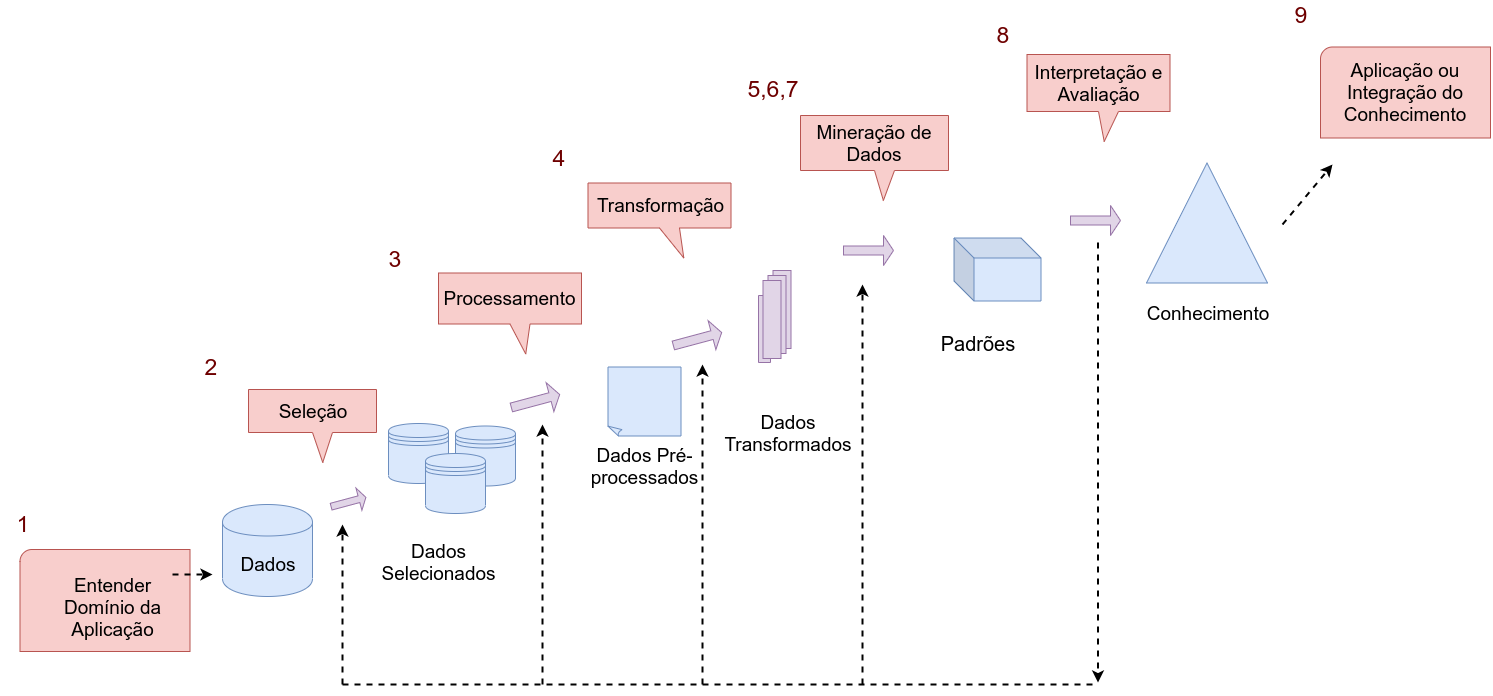
\includegraphics[scale=0.3]{preprojeto_Johnny/img/kdd_n.png}
      \caption{Etapas do Processo do processo de Descoberta de Conhecimento KDD. Adaptado de \cite{1996:Fayyad} e \cite{2014:Shafique}}
      \label{img:imag001}
    \end{figure}

    \begin{enumerate}
        % Etapa 01:
        \item \textbf{Entender o domínio da aplicação:}
        Fungos e suas características e importância para biodiversidade;
        % Etapa 02:
        \item \textbf{Criação da base de dados de interesse:}
        Como essa base de dados já está pronta, segue-se para próxima etapa do processo.
        % Etapa 03:
        \item \textbf{Limpeza de dados e pré processamento:}
        Realizar uma análise exploratória, utilizando métodos estatísticos. Segundo \citeonline{2009:Camilo}, alguns autores defendem que nessa fase do processo concentra-se de 50 a 80\% de todo volume de trabalho da pesquisa. Logo, essa etapa pode e deve ser considerada a principal dentre as demais. %Assim [citar fonte] define 4 subetapas que resultam no processo de entendimento dos dados:
    %     \begin{itemize}
    %         \item \textbf{Limpeza dos dados:}
    %         Eliminar problemas de registros incompletos, valores errados ou dados 
    % inconsistentes.
    %         \item \textbf{Integração dos dados:}
    %         Formar repositório único e consistente.
    %         \item \textbf{Transformação dos dados:}
    %         Pode-se ter necessidade de transformar valores numéricos em categóricos 
    % ou vice-versa, suavizar, sumarizar, agrupar, generalizar ou normalizar esses valores a fim de obter um modelo 
    % mais genérico ou mesmo um modelo melhor para dos dados colhidos.
    %         \item \textbf{Redução dos dados:} Análise de amostragem de volume de dados sem perder a representatividade do mesmo.
    %     \end{itemize}
        % Etapa 04:
        \item \textbf{Redução e Projeção de Dados:}
        Preocupa-se em encontrar atributos úteis dentro da base de dados, a depender do objetivo que se espera alcançar.
        % Etapa 05:
        \item \textbf{Escolha das funções de mineração:}
        Está diretamente relacionado ao propósito do modelo encontrado na fase de mineração.
        % Etapa 06:
        \item \textbf{Escolha dos algoritmos de mineração:}
        Os algoritmos escolhidos dependem do conhecimento que se espera obter e da forma como os dados foram tratados nas etapas anteriores.
        % Etapa 07:
        \item \textbf{Mineração:}
        Aplicação dos algoritmos de mineração.
        % Etapa 08:
        \item \textbf{Interpretação:}
        Análise dos resultados (Visualização). Testes, correções e validações.
        % Etapa 09:
        \item \textbf{Utilização do conhecimento descoberto:}
        Aplicação ou difusão do conhecimento obtido;
    \end{enumerate}
    
    % Importante destacar que as etapas do processo de Descoberta de Conhecimento são interativas e interativas, ou seja, estão intrinsecamente interligadas e podem/devem se repetir ao longo da pesquisa até que se obtenha resultados satisfatórios. %% citar imagem do diagrama de processo do KDD. %%% Finalizar/concluir texto base.

% ----------------------------------------- %
% Cronograma
% ----------------------------------------- %
\section*{Cronograma previsto de atividades}
\label{sec:crono}

\quad A descrição das atividades remanescentes está listada na Tabela \ref{tb:atividades}, enquanto que o cronograma é apresentado na Tabela \ref{tb:cronograma}.

%%%% INICIO ATIVIDADES PREVISTAS %%%%%%%%%%%%%%%%%

\setstretch{1} 
\begin{table}[!h]
  \centering
  \caption{Lista de atividades previstas.}\label{tb:atividades}
  \begin{tabular}{cp{9.4cm}}
    \hline \hline &\\[-0.4cm]
    {\bf Atividades} & \multicolumn{1}{c}{\bf Descrição} \\
    \hline
    &\\[-0.4cm]
    \textbf{A} &  Estudar os conceitos de: colônia, nicho, habitat e suas interações com a biodiversidade. \\[0.2cm]
    \textbf{B} &  Aplicar metodologia KDD para desenvolvimento do projeto.\\[0.2cm]
    \textbf{C} &  Estudar técnicas de mineração e visualização de dados.\\[0.2cm]
    \textbf{D} &  Estudar medidas de similaridades entre instâncias categóricas de objetos. \\[0.2cm]
    \textbf{E} &  Desenvolver aplicação web para registro e recuperação de dados para LAMBIO - UFT. \\[0.2cm]
    \textbf{F} &  Avaliar os modelos e padrões encontrados e caso necessário, voltar a D e refazer o processo até F.\\[0.2cm]
    \textbf{G} &  Aplicar técnicas de visualização e análise dos resultados.\\[0.2cm]
    \textbf{H} &  Aplicar medidas de avaliação dos resultados junto aos especialistas.\\[0.2cm]
    \textbf{I} &  Aplicar correções necessárias e distribuir os resultados com os envolvidos com a pesquisa e com a comunidade.\\[0.2cm]
    \textbf{J} &  Escrever monografia.\\[0.2cm]
    \hline \hline
  \end{tabular}
\end{table}

%%% FIM ATIVIDADES PREVISTAS %%%%%%%%%%%%%%%%%


%%%%% INICIO DO CRONOGRAMA %%%%%%%%%%%%%%

\begin{table}[!h]
  \centering \fontsize{8}{7}%\tiny
  \caption{Cronograma de Atividades}\label{tb:cronograma}
  \begin{tabular}{|c|c|c|c|c|c|c|}
    \hline
    {\normalsize\bf Ano}  & \multicolumn{6}{c|}{\normalsize\bf 2020}\\
    \hline
 {\normalsize\bf Mês} &
 \multirow{2}*{\bf Jan}&\multirow{2}*{\bf Fev}&\multirow{2}*{\bf Mar}&\multirow{2}*{\bf Abr}&\multirow{2}*{\bf Mai}&\multirow{2}*{\bf Jun}\\
   \cline{1-1}
{\bf Atv.}    & & & & & & \\
\hline
{\normalsize\bf A}  &$\surd$ & & & & & \\
\hline
{\normalsize\bf B} & &$\surd$ &$\surd$ &$\surd$ & $\surd$ &$\surd$ \\
\hline

{\normalsize\bf C} & &$\surd$ & & & & \\

\hline
{\normalsize\bf D} & & & &$\surd$ &$\surd$ & \\

\hline
{\normalsize\bf E} & & &$\surd$ &$\surd$ &$\surd$ &$\surd$ \\

\hline
{\normalsize\bf F} & & & & &$\surd$ & \\

\hline
{\normalsize\bf G} & & & & &$\surd$ & \\

\hline
{\normalsize\bf H} & & & & &$\surd$ & \\

\hline
{\normalsize\bf I} & & & & & &$\surd$\\

\hline
{\normalsize\bf J} &$\surd$ &$\surd$ &$\surd$ &$\surd$ &$\surd$ &$\surd$\\

\hline

  \end{tabular}
\end{table}


% ----------------------------------------------------------------------------------------------------- %
% Bibliografia
% ----------------------------------------------------------------------------------------------------- %
\bibliography{preprojeto_Johnny}

% --------------------------- %
% assinatura do Orientador
% ----------------------------%
% \begin{figure}[hbt]
%       % refazer imagem com observacao da etapa 0 - entendimento do dominio
%       % colocar tudo em portugues
%       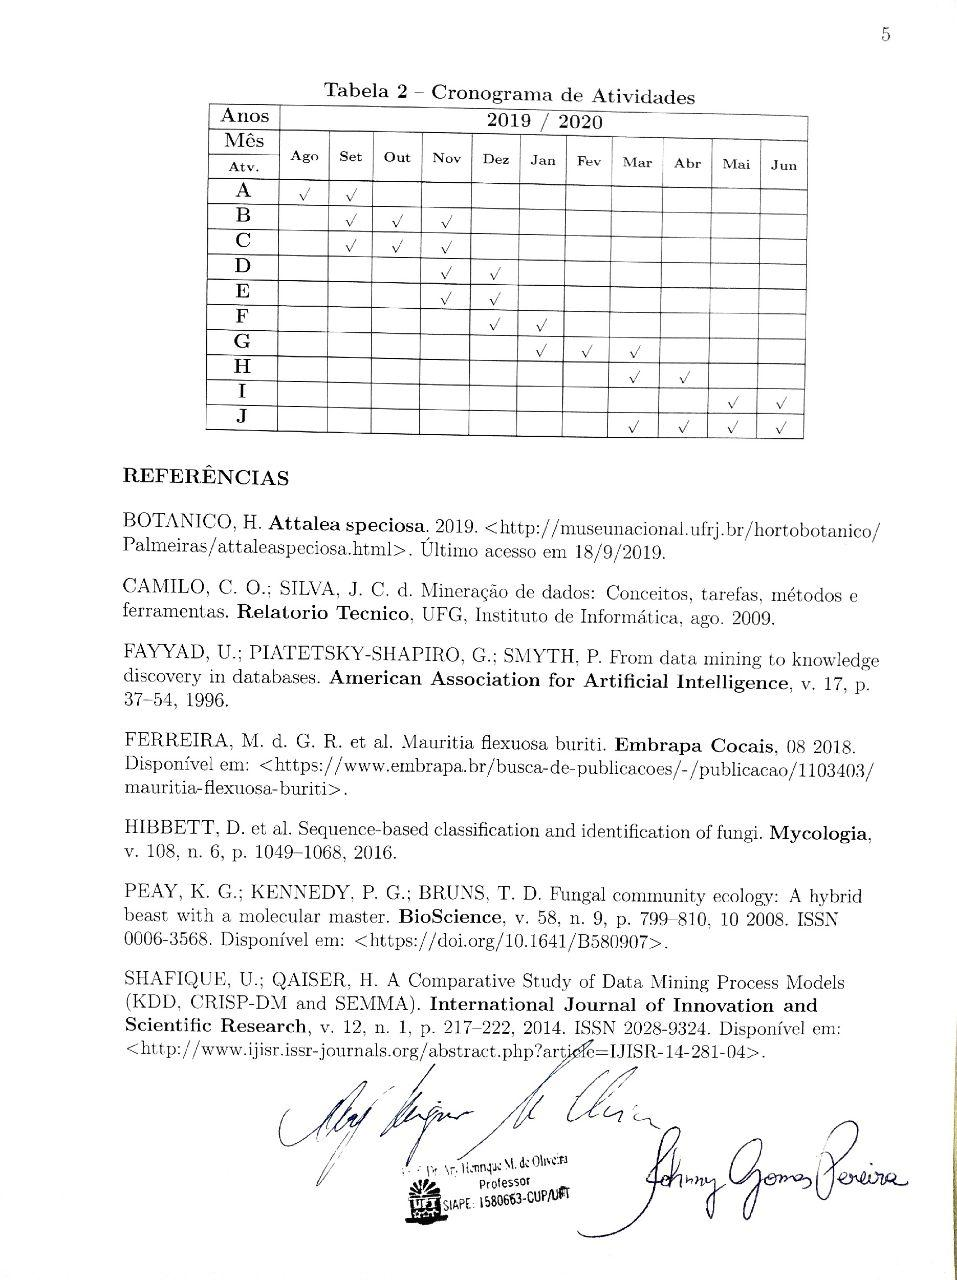
\includegraphics[scale=0.7]{preprojeto_Johnny/img/assinatura.jpg}
%       \label{img:imag002}
%     \end{figure}
% ----------------------------%

\end{document}
